\newpage
\section*{Задание 1}
\large

\addcontentsline{toc}{section}{\tocsecindent{Задание 1}}
\subsection*{Постановка задачи}
Вероятность некоторого случайного события равна 0.67. Сколько нужно произвести испытаний, чтобы с вероятностью 0.98 можно было ожидать, что наблюденная
частота этого события отклонится от его вероятности не более, чем на 0.01? Решить задачу,
используя неравенство Чебышева и интегральную теорему Муавра-Лапласа.
\subsection*{Решение}
Пусть случайная величина X - число появлений случайного события в n опытах. X имеет биномиальное распределение с параметрами $n$ и $p= 0.67$. Для биномиальной случайной величины математическое ожидание равно $np$, а дисперсия $np(1-p)$. Тогда
\begin{eqnarray}M(X)=np=0.67n \\ \nonumber D(X)=np(1-p)=n\cdot0.67\cdot0.33=0.2211n\end{eqnarray}
1) Используя неравенство Чебышева, 
\begin{equation}P\left(\left|X-M(X)\right|≤\epsilon\right) \geq \frac{1-D(X)}{\epsilon^2}\end{equation}
Получим:
\begin{eqnarray} P\left(\left|m-np\right|\leq 0.01n\right)=P\left(\left|X-M(X)\right|\leq 0.01n\right) \geq \frac{1-0.2211n}{(0.01n)^2} =1-\frac{2211}{n} \end{eqnarray}
\begin{eqnarray} \nonumber 1-\frac{2211}{n} \geq 0.98 \\ \frac{2211}{n} \leq 0.02 \\  n \geq \frac{2211}{0.02} = 110550 \end{eqnarray}
2) Решим эту же задачу, используя интегральную теорему Муавра—Лапласа (а точнее, следствие из нее),
\begin{eqnarray}
P \left( \left| {m} - np\right| \le \epsilon \right) \approx 	2\Phi\left(\frac{\epsilon}{\sqrt{np(1-p)}} \right)
\end{eqnarray}	
Подставим значения в формулу (6):
\begin{eqnarray}
P\left(\left| {m} - np\right| \le 0.01n\right)   = 	2\Phi\left( \frac{0.01n}{\sqrt{0.2211n}}\right) = 0.98\end{eqnarray}\begin{eqnarray} \nonumber
\Phi\left( \frac{0.01n}{\sqrt{0.2211n}}\right) = 0.49 \\
\frac{0.01n}{\sqrt{0.2211n}} \approx 2.33 \\
n = \frac{2.33^2 \cdot 0.2211}{0.01^2} \approx 12003.30
\end{eqnarray}
\textbf{Ответ:} $n \geq 110550$ из неравенства Чебышева, $n \geq 12004$ по теореме Муавара--Лапласа.

\section*{Задание 2}
\addcontentsline{toc}{section}{\tocsecindent{Задание 2}}
\subsection*{Постановка задачи}
С использованием метода моментов для случайной выборки $\overline{X} = (X_1, . . . , X_n)$ из генеральной
совокупности $X$ найти точечные оценки указанных параметров заданного закона распределения.
\begin{equation}
f_X(x) = 2\theta xe^{−\theta x^2}, x > 0
\end{equation}
\subsection*{Решение}
Найдем среднее выборочное:
\begin{eqnarray}
\overline{X} =  \int_0^\infty x \cdot 2\theta xe^{−\theta x^2}dx =  -\int_0^\infty xe^{−\theta x^2}d(-\theta x^2) = -\int_0^\infty x d(e^{-\theta x^2}) = \\ \nonumber =  \begin{vmatrix}
u = x  & du = dx \\ v = e^{-\theta x^2} & dv = d(e^{-\theta x^2}) 
\end{vmatrix} = -x \cdot e^{-\theta x^2} \bigg|_0^\infty + \int_0^\infty e^{-\theta x^2} dx	= \int_0^\infty e^{-\theta x^2} dx =  \\ \nonumber = \begin{vmatrix} t = \sqrt{2 \theta }x \\ x = \frac{t}{\sqrt{2\theta}} \\ dx = \frac{1}{\sqrt{2\theta}}dt\end{vmatrix} = \frac{1}{\sqrt{2\theta}} \int_0^\infty e^{-\frac{t^2}{2}}dt = \frac{1}{\sqrt{2\theta}} \cdot \sqrt{2\pi} \cdot \frac{1}{\sqrt{2\pi}} \int_0^\infty e^{-\frac{t^2}{2}}dt = \frac{1}{\sqrt{2\theta}} \cdot \sqrt{2\pi} \cdot \frac{1}{2} = \frac{\sqrt\pi}{2\sqrt\theta} 
\end{eqnarray}
Откуда получаем, что \begin{eqnarray}\theta = (\frac{\sqrt\pi}{2\overline{X}})^2\end{eqnarray} \\
\textbf{Ответ:} $\theta = (\frac{\sqrt\pi}{2\overline{X}})^2$

\section*{Задание 3}
\addcontentsline{toc}{section}{\tocsecindent{Задание 3}}
\subsection*{Постановка задачи}
С использованием метода максимального правдоподобия для случайной выборки $\overline{X} = (X_1, . . . , X_n)$ из генеральной совокупности X найти точечные оценки параметров заданного
закона распределения. Вычислить выборочные значения найденных оценок для выборки $\overline{x_5} = (x_1, . . . , x_n)$
\begin{eqnarray}
f_X(x) = \frac{\theta}{x^{\theta+1}}, x>1 \\
\overline{x_5} = (e, e^2,e^3,e^4,e^5)
\end{eqnarray}
\subsection*{Решение}
Получим функцию правдоподобия для нашей выборки $\overline{x_5}$:
\begin{eqnarray}
L(X_1,...,X_n, \theta) = P \{X=X_1\} \cdot ... \cdot P \{X=X_n\} = \theta^5 \cdot \frac{1}{e^{\theta+1}} \cdot \frac{1}{e^{2(\theta+1)}} \cdot \frac{1}{e^{3(\theta+1)}} \cdot \frac{1}{e^{4(\theta+1)}} \cdot \\ \nonumber \cdot \frac{1}{e^{5(\theta+1)}} = \theta^5 \cdot\frac{1}{e^{15(\theta+1)}}
\end{eqnarray}
Прологарифмируем ее:
\begin{eqnarray}
lnL(X_1,...,X_n, \theta) = ln \left(\theta^5 \cdot\frac{1}{e^{15(\theta+1)}}\right) = ln(\theta^5) + ln\left(\frac{1}{e^{15(\theta+1)}}\right) = 5ln\theta - 15(\theta+1)
\end{eqnarray}
Необходимое условие экстремума $L(\overline{X}, \theta)$:
\begin{equation}
\frac{dlnL}{d\theta}=0
\end{equation}
Продифференцируем (12):
\begin{equation}
\frac{dlnL}{d\theta}=\frac{d(5ln\theta - 15(\theta+1))}{d\theta} =\frac{5}{\theta}-15
\end{equation}
Приравняв к нулю, получим, что
\begin{equation}
{\theta}=\frac{1}{3}
\end{equation}
\textbf{Ответ:} ${\theta}=\frac{1}{3}$

\section*{Задание 4}
\addcontentsline{toc}{section}{\tocsecindent{Задание 4}}
\subsection*{Постановка задачи}
По результатам $n = 25$ измерений скорости снаряда получена оценка дисперсии $S^2(\overline{X_n}) = 5.8 м/c^2$. Считая распределение контролируемого признака нормальным, построить $90\%-ые$ доверительные интервалы для дисперсии и среднего квадратичного отклонения скорости снаряда.
\subsection*{Решение}
Построим доверительный интервал для дисперсии скорости снаряда, используя центральную статистику:
\begin{equation}
T(\vec{X}, \sigma^2) = \frac{S^2(\overline{X_n})}{\sigma^2}(n-1) \sim \chi^2(n-1)
\end{equation}
Ниже изображен график функции плотности распределения статистики $T$. 
\begin{figure}[h!]
	\caption{График функции плотности распределения статистики $T$}
	\center 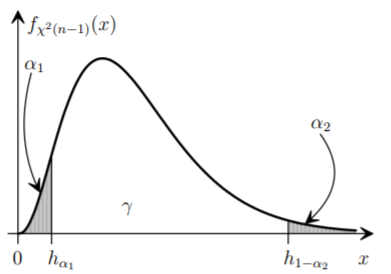
\includegraphics{img/1.png}
\end{figure}\\
В соответствии со свойствами непрерывных случайных величин,
\begin{equation}
\gamma = P\left\{ h_{\frac{1-\alpha}{2}} < T(\vec{X}, \sigma^2) < h_{\frac{1+\alpha}{2}}\right\}
\end{equation}
Подставим формулу (20) для $T(\vec{X}, \sigma^2)$:
\begin{equation}
\gamma = P\left\{ h_{0.05} < \frac{S^2(\overline{X_n})}{\sigma^2}(n-1) < h_{0.95}\right\}
\end{equation}
\begin{equation}
\gamma = P\left\{ \frac{S^2(\overline{X_n})}{h_{0.05}}(n-1) < \sigma^2 < \frac{S^2(\overline{X_n})}{h_{0.95}}(n-1)\right\}
\end{equation}
Откуда получим 90\%-ый доверительный интервал для дисперсии снаряда:
\begin{equation}
0.9 = P\left\{ 3.82 < \sigma^2 <10.05\right\}
\end{equation}
Соответственно, 90\%-ый доверительный интервал для среднего квадратичного отклонения скорости снаряда:
\begin{equation}
\nonumber 0.9 = P\left\{ \sqrt{3.82} < \sigma <\sqrt{10.05}\right\}
\end{equation}
\begin{equation}
0.9 = P\left\{ 1.95 < \sigma <3.17\right\}
\end{equation}
\textbf{Ответ:} $\sigma^2 \in (3.82;10.05) \frac{\text{м}}{c^2}$; $\sigma \in (1.95;3.17) \frac{\text{м}}{c}$. 